\chapter{Molecular Approximations}
\label{c:molecular_approximations}

\section{The Rigid Rotator}
\label{s:the_rigid_rotator}

\subsection{Theory}

The rigid rotator model assumes that the molecule is shaped like a dumbbell. Each of the two atoms of masses $m_1$ and $m_2$ is point-like and are affixed to one another via a massless rigid rod of radius $r$.

\begin{figure}[H]
    \centering
    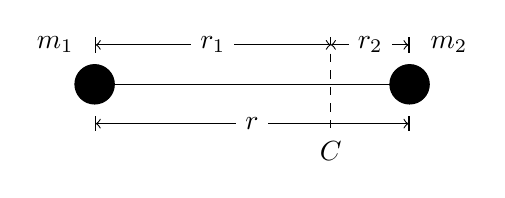
\begin{tikzpicture}
        \draw[fill=black](-2,0) circle(0.25);
        \node at (-2.5,0.5){$m_1$};
        \draw[color=black] (-2,0)rectangle(2,0);
        \draw[fill=black] (2,0)circle(0.25);
        \node at (2.5,0.5){$m_2$};

        \draw[|<->|](-2,-0.5)--(2,-0.5) node[midway, fill=white]{$r$};
        \draw[dashed](1,0.6)--(1,-0.6) node[below]{$C$};
        \draw[|<->](-2,0.5)--(1,0.5) node[midway, fill=white]{$r_1$};
        \draw[<->|](1,0.5)--(2,0.5) node[midway, fill=white]{$r_2$};
    \end{tikzpicture}
    \caption{Dumbbell model of a diatomic molecule.}
    \label{f:dumbbell_model}
\end{figure}

The classical expression for the rotational energy of a rigid body is
\begin{equation*}
    E = \frac{1}{2}I\omega^2,
\end{equation*}
where $\omega$ is the angular velocity and $I$ is the moment of inertia of the body about the axis of rotation $C$. For a point mass, the moment of inertia about an axis of a body is
\begin{equation*}
    I = \sum_i m_i r_i^2.
\end{equation*}
Using this definition, the magnitude of the angular momentum of the system can be found as
\begin{equation*}
    L = I\omega.
\end{equation*}
Using the angular momentum, the rotational energy of the system can now be expressed as
\begin{equation*}
    E = \frac{L^2}{2I}.
\end{equation*}

For the dumbbell model, the moment of inertia is
\begin{equation*}
    I = m_1r_1^2 + m_2r_2^2,
\end{equation*}
where
\begin{equation*}
    r_1 = \frac{m_2}{m_1 + m_2}r \quad\text{and}\quad r_2 = \frac{m_1}{m_1 + m_2}r
\end{equation*}
are the distances of the two masses $m_1$ and $m_2$ from the center of gravity $C$. Substituting these two expressions into the moment of inertia gives
\begin{equation*}
    I = \mu r^2,
\end{equation*}
where
\begin{equation*}
    \mu = \frac{m_1m_2}{m_1 + m_2}
\end{equation*}
is the reduced mass of the molecule.

\subsection{Energy Levels}

The appropriate Schr\"odinger Equation for the rigid rotator has $m = \mu$ and $V = 0$ since the model is regarded as perfectly rigid. Solving
\begin{equation*}
    \odv[2]{\psi}{x} + \pdv[2]{\psi}{y} + \pdv[2]{\psi}{z} + \frac{8\pi^2\mu}{h^2}E\psi = 0
\end{equation*}
leads to the energy eigenvalues given by
\begin{equation*}
    E = \frac{h^2J(J + 1)}{8\pi^2\mu r^2} = \frac{h^2J(J + 1)}{8\pi^2I},
\end{equation*}
where $J$ is the rotational quantum number. The quantized angular momentum can be found using the classical formula shown earlier, which leads to
\begin{equation*}
    L = \sqrt{2EI} = \frac{h}{2\pi}\sqrt{J(J + 1)}.
\end{equation*}
The angular velocity $\omega$ and rotational frequency $\nu\_{rot}$ can also be found as
\begin{equation*}
    \omega = \frac{h}{2\pi I}\sqrt{J(J + 1)} \quad\text{and}\quad \nu\_{rot} = \frac{\omega}{2\pi} = \frac{h}{4\pi^2I}\sqrt{J(J + 1)}.
\end{equation*}

\subsection{Spectrum}

The emission of a light quantum results from the transition of the rotator from a higher to a lower energy level. Conversely, the absorption of a light quantum produces a transition from a lower to a higher level. The wave number $\nu$ of the emitted or absorbed quantum is
\begin{equation*}
    \nu = \frac{E'}{hc} - \frac{E''}{hc}.
\end{equation*}
The single prime $'$ refers to the upper state, while the double prime $''$ refers to the lower state.

The quantity $E/hc$ is called the rotational term value and is denoted $F(J)$. The value of $F(J)$ is given as
\begin{equation*}
    F(J) = \frac{E}{hc} = \frac{h}{8\pi^2cI}J(J + 1) = BJ(J + 1).
\end{equation*}
The constant
\begin{equation*}
    B = \frac{h}{8\pi^2cI}
\end{equation*}
is called the rotational constant and is essentially the reciprocal moment of inertia. These two definitions allow for the rewriting of the wavenumber as
\begin{equation*}
    \nu = F(J')- F(J'') = BJ'(J' + 1) - BJ''(J'' + 1).
\end{equation*}

To find which frequencies are actually emitted or absorbed, selection rules for the rotational quantum number $J$ must be established. The selection rule for $J$ is
\begin{equation*}
    J' = J'' \pm 1; \quad\text{that is,}\quad \Delta{}J = J' - J'' = \pm 1.
\end{equation*}

Because $J' > J''$ always (due to $J'$ being the upper state), only $\Delta{}J = +1$ needs to be considered. Therefore, the absorbed or emitted lines of the rigid rotator are given by
\begin{equation*}
    \nu = F(J'' + 1) - F(J'') = B(J'' + 1)(J'' + 2) - BJ''(J'' + 1) = 2B(J'' + 1).
\end{equation*}
Writing $J$ instead of $J''$ when only the $J$ value of the lower state occurs, we get
\begin{equation*}
    \nu = 2B(J + 1) \quad\text{for}\quad J = 0, 1, 2, \dotsb.
\end{equation*}
The rotational frequency of the rigid rotator is
\begin{equation*}
    \nu\_{rot} = 2cB\sqrt{J(J + 1)}.
\end{equation*}

\section{The Harmonic Oscillator}
\label{s:the_harmonic_oscillator}

\subsection{Theory}

In classical mechanics, the equation of motion for a simple harmonic oscillator is
\begin{equation*}
    F = -kx = m\odv[2]{x}{t},
\end{equation*}
where $F$ is the force experienced by the particle toward the equilibrium position which is proportional to the distance $x$ away from the equilibrium position. Solving the differential equation for $x$ yields
\begin{equation*}
    x = x_0\sin(2\pi t\nu\_{vib} + \varphi),
\end{equation*}
where the vibrational frequency $\nu\_{vib}$ is given by
\begin{equation*}
    \nu\_{vib} = \frac{1}{2\pi}\sqrt{\frac{k}{m}}.
\end{equation*}

The potential energy for a linear spring is
\begin{equation*}
    V = \frac{1}{2}kx^2 = 2\pi^2mx^2\nu\_{vib}^2
\end{equation*}

The restoring force exerted by the two atoms in a molecule after being displaced from their equilibrium position $r_e$ can be modeled by the equation of motion for a spring as
\begin{equation*}
    m_1\odv[2]{r_1}{t} = -k(r - r_e)
\end{equation*}
and
\begin{equation*}
    m_2\odv[2]{r_2}{t} = -k(r - r_e).
\end{equation*}
Substituting $r$ in place of both $r_1$ and $r_2$ gives the single equation
\begin{equation*}
    \frac{m_1m_2}{m_1 + m_2}\odv[2]{r}{t} = -k(r - r_e),
\end{equation*}
which is equivalent to
\begin{equation*}
    \mu\odv[2]{(r - r_e)}{t} = -k(r - r_e)
\end{equation*}
since $r_e$ is constant. From direct comparison with the classical equation of motion for a harmonic oscillator, it follows that the vibrational frequency of the molecule is
\begin{equation*}
    \nu\_{vib} = \frac{1}{2\pi}\sqrt{\frac{k}{\mu}}.
\end{equation*}

\subsection{Energy Levels}

The Schr\"odinger equation for the harmonic oscillator is
\begin{equation*}
    \odv[2]{\psi}{x} + \frac{8\pi^2\mu}{h^2}\pr*{E - \tfrac{1}{2}kx^2}\psi = 0.
\end{equation*}
Solving this equation leads to the energy eigenvalues given by
\begin{equation*}
    E(v) = \frac{h}{2\pi}\sqrt{\frac{k}{\mu}}\pr*{v + \tfrac{1}{2}} = h\nu\_{vib}\pr*{v + \tfrac{1}{2}} \quad\text{for}\quad v = 0, 1, 2, \dotsb.
\end{equation*}
Rewriting the energy as the vibrational term value $G(v)$ gives
\begin{equation*}
    G(v) = \frac{E(v)}{hc} = \frac{\nu\_{vib}}{c}\pr*{v + \tfrac{1}{2}} = \omega\pr*{v + \tfrac{1}{2}},
\end{equation*}
where the quantity $\nu\_{vib}/c$ is designated $\omega$ and measured in \unit{cm^{-1}}.

\subsection{Spectrum}

Similarly to the rigid rotor, the wavenumber of the emitted or absorbed light is given by
\begin{equation*}
    \nu = \frac{E(v')}{hc} - \frac{E(v'')}{hc} = G(v') - G(v''),
\end{equation*}
where $v'$ and $v''$ are the quantum numbers of the upper and lower state, respectively.

The selection rule for the vibrational quantum number of the harmonic oscillator is
\begin{equation*}
    \Delta{}v = v' - v'' = \pm 1.
\end{equation*}
Again denoting $J''$ as $J$, the wavenumber of the emitted or absorbed light is
\begin{equation*}
    \nu = G(v + 1) - G(v) = \omega.
\end{equation*}

\section{The Anharmonic Oscillator}
\label{s:the_anharmonic_oscillator}

\subsection{Theory}

A first approximation to the actual potential energy function of the molecule can be written as
\begin{equation*}
    U = f(r - r_e)^2 - g(r - r_e)^3,
\end{equation*}
where $f$ and $g$ are coefficients, with $g$ being much smaller than $f$. Better approximations can be made by adding higher order terms to this expression.

The motion of the anharmonic oscillator can be represented as a superposition of fundamental and overtone vibrations as the following Fourier series:
\begin{equation*}
    x = x_{01}\sin{2\pi\nu\_{vib}t} + x_{02}(3 + \cos{2\pi2\nu\_{vib}t}) + x_{03}\sin{2\pi3\nu\_{vib}t} + \dotsb.
\end{equation*}
In this expression, $x_{01}$, $x_{02}$, and $x_{03}$ are the amplitudes of the fundamental, the first, and the second overtone, respectively. If the anharmonicity is small $(g \ll f)$, then $x_{02} \ll x_{01}$ and $x_{03} \ll x_{02}$. However, $x_{02}$ and $x_{03}$ are proportional to the square and cube of $x_{01}$, respectively and rapidly become more important as $x_{01}$ increases. Because of the asymmetric potential curve, the time average of the position is not at $x = 0$, but instead at $x = 3x_{02}$.

The frequency of the vibrations is given as
\begin{equation*}
    \nu\_{vib} = \frac{1}{2\pi}\sqrt{\frac{k}{\mu}}
\end{equation*}
for very small amplitudes only. This factor decreases slowly as the amplitude $x_{01}$ increases.

\subsection{Energy Levels}

Substituting the anharmonic potential energy function into the Schr\"odinger equation and solving for the energy eigenvalues gives
\begin{equation*}
    E_v = hc\omega_e\pr*{v + \tfrac{1}{2}} - hc\omega_ex_e\pr*{v + \tfrac{1}{2}}^2 + hc\omega_ey_e\pr*{v + \tfrac{1}{2}}^3 + \dotsb.
\end{equation*}
Written as the vibrational term $G(v)$, this becomes
\begin{equation*}
    G(v) = \omega_e\pr*{v + \tfrac{1}{2}} - \omega_ex_e\pr*{v + \tfrac{1}{2}}^2 + \omega_ey_e\pr*{v + \tfrac{1}{2}}^3 + \dotsb,
\end{equation*}
where $v$ is the vibrational quantum number, $\omega_ex_e \ll \omega_e$, and $\omega_ey_e \ll \omega_ex_e$. This equation directly shows that the energy levels of the anharmonic oscillator are not equidistant like those of the harmonic oscillator.

The zero-point energy of the anharmonic oscillator is given by setting $v = 0$ in the vibrational term above:
\begin{equation*}
    G(0) = \tfrac{1}{2}\omega_e - \tfrac{1}{2}\omega_ex_e + \tfrac{1}{8}\omega_ey_e + \dotsb.
\end{equation*}

\subsection{Spectrum}

The selection rule for the anharmonic oscillator is given by
\begin{equation*}
    \Delta{}v = \pm 1
\end{equation*}
for the most intense transitions, but the two selection rules of
\begin{equation*}
    \Delta{}v = \pm 2 \quad\text{and}\quad \Delta{}v = \pm 3
\end{equation*}
can also appear with decreasing intensity.

The formula for the series of absorption bands $1\dash0$, $2\dash0$, $3\dash0$, $\dotsb$ is given as
\begin{equation*}
    \nu\_{abs} = G(v') - G(0) = G_0(v') = \omega_0v' - \omega_0x_0v'^2 + \omega_0y_0v'^3 + \dotsb.
\end{equation*}

\section{The Nonrigid Rotator}
\label{s:the_nonrigid_rotator}

\subsection{Energy Levels}

A good approximation shows that the rotational terms of the nonrigid rotator are given by
\begin{equation*}
    F(J) = \frac{E_r}{hc} = B[1 - uJ(J + 1)]J(J + 1),
\end{equation*}
where the value $B[1 - uJ(J + 1)]$ now appears in the place of $B$ in the equation for the rigid rotator. This equation can also be written as
\begin{equation*}
    F(J) = BJ(J + 1) - DJ^2(J + 1)^2,
\end{equation*}
where $D$ always has a positive value with this choice of sign. If cubic and higher powers in the potential energy are included, the rotational terms values are
\begin{equation*}
    F(J) = BJ(J + 1) - DJ^2(J + 1)^2 + HJ^3(J + 1)^3 + \dotsb.
\end{equation*}

\subsection{Spectrum}

The selection rule for the infrared spectrum of the rigid rotator $\Delta{}J = \pm 1$ is also valid for the nonrigid rotator. Therefore, the wavenumbers of the lines of the infrared rotation spectrum are
\begin{equation*}
    \nu = F(J + 1) - F(J) = 2B(J + 1) - 4D(J + 1)^3.
\end{equation*}

\section{The Vibrating Rotator}
\label{s:the_vibrating_rotator}

\subsection{Energy Levels}

Since the molecule is vibrating, the internuclear distance and therefore the moment of inertia and the rotational constant $B$ are changing rapidly. Since the period of vibration is small compared to the period of rotation, the mean value of $B$ is
\begin{equation*}
    B_v = \frac{h}{8\pi^2c\mu}\bk*{\bar{\frac{1}{r^2}}},
\end{equation*}
where $\overline{1/r^2}$ is the mean value of $1/r^2$ during the vibration. The value of $B_v$ will be expected to be smaller than the equilibrium constant $B_e$ since the mean nuclear separation will be greater. The value of $B_e$ is given by
\begin{equation*}
    B_e = \frac{h}{8\pi^2c\mu{}r_e^2} = \frac{h}{8\pi^2cI_e}.
\end{equation*}
To a first approximation, the rotational constant $B_v$ in the vibrational state $v$ is given as
\begin{equation*}
    B_v = B_e - \alpha_e\pr*{v + \tfrac{1}{2}} + \dotsb,
\end{equation*}
where $\alpha_e$ is a constant which is small compared to $B_e$. The ratio $\alpha_e/B_e$ is only slightly larger than $\omega_ex_e/\omega_e$.

A mean rotational constant $D_v$ representing the contribution of centrifugal force can be found as
\begin{equation*}
    D_v = D_e + \beta_e\pr*{v + \tfrac{1}{2}} + \dotsb.
\end{equation*}
In this equation, $\beta_e$ is small compared to
\begin{equation*}
    D_e = \frac{4B_e^3}{\omega_e^2}.
\end{equation*}

The rotational terms in a given vibrational level are therefore given by
\begin{equation*}
    F_v(J) = B_vJ(J + 1) - D_vJ^2(J + 1)^2 + \dotsb.
\end{equation*}
Taking into account the interaction between vibration and rotation, the term values for the vibrating rotator are
\begin{equation*}
    T = G(v) + F_v(J) = \omega_e\pr*{v + \tfrac{1}{2}} - \omega_ex_e\pr*{v + \tfrac{1}{2}}^2 + \dotsb + B_vJ(J + 1) - D_vJ^2(J + 1)^2 + \dotsb.
\end{equation*}
For the lowest vibrational state $v = 0$, the rotational constant $B_0$ must be used in this equation.

If very precise measurements are available, higher powers of $\pr*{v + \tfrac{1}{2}}$ can be taken into account using
\begin{equation*}
    B_v = B_e - \alpha_e\pr*{v + \tfrac{1}{2}} + \gamma_e\pr*{v + \tfrac{1}{2}}^2 + \dotsb.
\end{equation*}
In higher powers of $J(J + 1)$, the rotational term can be expressed as
\begin{equation*}
    F_v(J) = B_vJ(J + 1) - D_vJ^2(J + 1)^2 + H_vJ^3(J + 1)^3 + \dotsb,
\end{equation*}
where the rotational constant $H_v$ is given as
\begin{equation*}
    H_v \approx H_e = \frac{2D_e}{3\omega_e^2}(12B_e^2 - \alpha_e\omega_e)
\end{equation*}
to a first approximation.

\section{The Symmetric Top}
\label{s:the_symmetric_top}

\subsection{Theory}

\subsection{Energy Levels}

\subsection{Spectra}
